\documentclass[xcolor=dvipsnames]{beamer}
\usepackage{amsmath}
\usepackage{hyperref}
\usepackage{ragged2e}
\usetheme{Copenhagen}
\usecolortheme[named=Black]{structure}

\title{SURF: Speeded-Up Robust Features}
\author{Castleberry, Cherry, and Firth}
\renewcommand{\raggedright}{\leftskip=0pt \rightskip=0pt plus 0cm}

\begin{document}

% Camera calibration and object recognition.
\section{Introduction and Overview}
\subsection{Motivation}
\frame{ \frametitle{Motivation}
\begin{itemize}
 \item The motivation is to facilitate advances in:
 \begin{itemize}
  \item Image registration
  \item Camera calibration 
  \item Object recognition
  \item Image retrieval 
 \end{itemize} 
\end{itemize} 
}

\subsection{Problem Definition}
\frame{ \frametitle{Problem Definition}
\begin{itemize}
 \item The problem is to efficiently and accurately find point correspondences between two images depicting the same scene, thereby enabling camera calibration and object recognition.
 \item The problem solution is subdivided into three stages:
 \begin{itemize}
  \item \textbf{Detection}: identify points of interest. The most important aspect of a detector is its repeatability.
  \item \textbf{Description}: create a vector which holds data about the feature(s). It should be simple (low-dimensional) to facilitate efficient matching but complex enough to adequately describe the feature.
  \item \textbf{Matching}: match the feature vectors across images. The matching is based on a distance measure between the two feature vectors (such as the \hyperlink{math-distance}{\beamergotobutton{Mahalanobis or Euclidean distance}}).
  %ex_euc_dist.fw.png
  %ex_mah_dist.fw.png
 \end{itemize} 
\end{itemize} 
}

\frame{ \frametitle{Problem Definition}
%ex_geo_photo_diffs.fw.png
\begin{itemize}
 \item The goal is to develop a detector and descriptor which, in comparison to the state-of-the-art detectors and descriptors of the day, are computationally inexpensive but do not sacrifice performance (accuracy of matches).
 \item The focus is on scale and in-plane rotation invariant detectors and descriptors. The descriptor is robust enough to handle skew, anisotropic scaling (stretching), and perspective effects.
 \item The handling of photometric deformations is limited to bias (offset, or brightness changes) and contrast changes (by a scale factor).
\end{itemize} 
}

\subsection{Previous Work}
\frame{ \frametitle{Previous Work - Interest Point Detection}
Harris corner detector
 \begin{itemize}
  \item Uses eigenvalues of second moment matrix
  \item Not scale invariant
 \end{itemize}

Lindeburg
 \begin{itemize}
  \item Introduced concept of automatic scale selection
  \item Experimented with the determinant of the Hessian matrix and the Laplacian
 \end{itemize}

Mikolajczyk and Schmid
 \begin{itemize}
  \item Harris-Laplace or Hessian-Laplace
  \item Scale invariant feature detection with high repeatability
  \item Used determinant of the Hessian matrix to select location, and Laplacian to select scale
 \end{itemize}
}

\frame{ \frametitle{Previous Work - Interest Point Detection}
Lowe
 \begin{itemize}
  \item Used a Difference of Gaussians filter to approximate a Laplacian of Gaussians
 \end{itemize}
 
 Conclusions from previous work on interest point detection:
 Hessian-based detectors are more stable and repeatable than their Harris-based counterparts. Also, approximations such as DoG provide good speed with minimal loss in  accuracy.
}

\frame{ \frametitle{Previous Work - Interest Point Description}
Many interest point description techniques exist, including: Gaussian derivatives, moment invariants,  complex features, steerable filters, phase-based local features...

Lowe (SIFT)
 \begin{itemize}
  \item Computes a histogram of local oriented gradients around the interest point and stores the bins in a 128-dimensional vector
 \end{itemize}

Ke and Sukthankar (PCA-SIFT)
 \begin{itemize}
  \item Apply PCA to the gradient image around the interest point
  \item 36-dimensional descriptor vector is faster in matching but less distinctive than SIFT
  \item Also proposes GLOH, but is similarly computationally expensive due to it's use of PCA
 \end{itemize}
 
Grabner
 \begin{itemize}
  \item Used integral images to approximate SIFT
 \end{itemize}
}

\subsection{Background}
\frame{ \frametitle{Background}
 \begin{itemize}
 \item Detection of interest points is done through approximations of the \hyperlink{math-laplacian}{\beamergotobutton{Laplacian}} of \hyperlink{math-gaussian}{\beamergotobutton{Gaussians}}, then finding extrema within the scale space of the image. 
 \item Description is handled by assigning orientation vectors using \hyperlink{math-haar}{\beamergotobutton{Haar wavelets}} over a 4x4 grid. Four values ($d_x, d_y, |d_x|, |d_y|$) are stored for each cell, yielding a 64-dimension description vector.
 \item Matching is facilitated by indexing the results with the sign of the Laplacian, which indicates if the blob is block-on-white or white-on-black. The nearest-neighbor ratio matching is used.
 \end{itemize} 
}

\section{Description of the Method} \subsection{Techniques Used}
  
\frame{ \frametitle{Blob Detection}
\begin{itemize}
\item To summarize the method: an
\hyperlink{math-integral}{\beamergotobutton{integral image}} is first
calculated on the image I(x,y), which facilitates the subsequent approximation of the
\hyperlink{math-determinant}{\beamergotobutton{determinant}} of the
\hyperlink{math-hessian}{\beamergotobutton{Hessian matrix}} for the image 
$(x,y)$ over its scale space. The scale space is constructed not by taking
%eqn_basic_hessian.fw.png
%ex_basic_hessian.fw.png
\hyperlink{math-gaussian}{\beamergotobutton{Gaussians}} of increasing scales
and downsampling as in SIFT, but instead by convolving with the image box
filters (of increasing size) which approximate the
\hyperlink{math-hessian}{\beamergotobutton{Laplacian}} of Gaussians.  Extrema
of the Hessian determinants found within the \textbf{octaves} constituting the
scale space of the image indicate blob responses.
\end{itemize} 
}

\frame{ \frametitle{Orientation Assignment}
\begin{itemize} 
\item The \hyperlink{math-haar}{Haar wavelet} responses for each point within a
neighboorhood of $6s$ (where $s$ is the image scale) are calculated by
convolving a Haar wavelet filter of $4s$ over the image. The wavelet responses
are weighted with a Gaussian ($\sigma = 2s$) at the center of the interest
point. Haar responses ($x_h, y_h$) within a circle of $6s$ around the interest
point are graphed.  Haar responses within a window of $\theta$ to
$\theta+\frac{\pi}{3}$ are summed for $\theta$ from $0$ to $2 \pi$ to form an
orientation vector for that value of $\theta$.  The maximum of these Haar
response vectors is taken to give the dominant orientation for the interest
point.
\end{itemize} 
}

\subsection{Method}
\frame{ \frametitle{Hessian Approximation}
 \begin{itemize} 
  \item A \hyperlink{math-hessian}{\beamergotobutton{Hessian Matrix}} is approximated using box filters. The box filters are approximations of second-order derivatives of Gaussians within a rectangular region. These approximations are efficiently computed using \hyperlink{math-integral}{\beamergotobutton{integral images}}.
  \item The determinant of the Hessian matrix is approximated using the box filters:
\begin{equation}
  det_{approx}(\mathcal{H}) = D_{xx} D_{yy} - (wD_{xy})^2
\end{equation}
  \item where $w$ is a weight needed to adjust for the difference between the approximated and actual Gaussian.
  \end{itemize}
}

\frame{ \frametitle{Hessian Determinant Approximation}
 \begin{itemize} 
  \item $w$ for an $n$x$n$ box filter approximating a Gaussian with $\sigma$ is equal to:
 \begin{equation}
  \frac{
  {|L_{xy}(\sigma)|_F}/{|L_{yy}(\sigma)|_F}}{
  {|D_{xy}(n)|_F}/{|D_{yy}(n)|_F} }
 \end{equation}
 where $|x|_F$ is the
 \hyperlink{math-frobenius}{\beamergotobutton{Frobenius norm}}. This factor changes with filter size; however, it is desirable to keep it constant. Therefore the filter responses ($D$) are normalized with respect to their size to guarantee a constant Frobenius norm. 
 %ex_frobenius_norm.fw.png
 \item The $det_{approx}$ represents a \emph{blob response} in $I$ at $\mathbf{x}$. $det_{approx}$ for all locations $\mathbf{x}$ in the image gives a \emph{blob response map}. Local maxima are detected to give the locations of blobs.
 \end{itemize} 
}

\frame{ \frametitle{Scale Spaces}
 \begin{itemize}
  \item Interest points should be found at different scales. To represent the image at different scales, a \textbf{scale pyramid} is used. 
  \item Rather than iteratively reducing the size of the image, the box filters are
upscaled and computed, for which there is little additional computational cost. As a side effect of not downsampling the image, there is no \textbf{aliasing}. As a downside of this approach, up-scaled box filters can lose high-frequency components, which can limit scale-invariance.
  \item A scale space is divided into \textbf{octaves}. 
 \end{itemize} 
}

\frame{ \frametitle{Octaves}
 \begin{itemize}
  \item An octave represents a series of filter response maps obtained by 
\hyperlink{math-convolution}{\beamergotobutton{convolving}} the same input image with a filter of increasing size.  
  \item The octave encompasses a scaling factor of 2. The pixel difference between scales of the image is at least one-third of the filter size (which is the size of the lobes in $D_{xx}$ or $D_{yy}$). For odd-$n$ filter sizes, a minimum of 2 pixels is required to guarantee a central pixel. In the case of a filter of size 9, this amounts to a difference of 6.
 \end{itemize} 
}

\frame{ \frametitle{Scale Interpolation}
 \begin{itemize}
  \item To localize interest points in the image over scales, non-maximum suppression in a 3x3x3 neighboorhood is applied (Neubeck and Van Gool).
  \item The maxima of the determinant of the Hessian matrix are then interpolated in scale and image space (Brown et al).
 \end{itemize} 
}

\frame{ \frametitle{Interest Point Description}
 \begin{itemize}
  \item Similar to SIFT, the SURF describes the distribution of the intensity within the interest point neighoorhood, but with first-order \hyperlink{math:haar}{\beamergotobutton{Haar wavelet}} responses in the $x$ and $y$ dimensions rather than the gradient.
  \item Also, integral images are exploited for efficiency, and only 64 dimensions are used.
 \end{itemize} 
}

\frame{ \frametitle{Orientation Assignment}
 \begin{itemize}
  \item For the interest points to be rotation-invariant, the orientation must be reproducible. Haar wavelet responses are calculated in the $x$ and $y$ directions within a circular neighboorhood of radius $6s$, where $s$ is the scale factor. 
  \item Integral images are used for fast filtering. Only six operations are required to compute the Haar wavelet response in $x$ or $y$ for any $s$.
  \item The Haar wavelet responses are weighted with a Gaussian ($\sigma = 2s$) centered at the interest point. They are represented as points ($x_{Haar}, y_{Haar}$) where $x_{Haar}$ represents the magnitude of the horizontal response and $y_{Haar}$ represents magnitude of the vertical response.
  \item The circle is divided into slides of $\frac{pi}{3}$ and the Haar responses are summed for each slice to give a local orientation vector. 
 \end{itemize} 
}

\frame{ \frametitle{}
}

\subsection{Data}
\frame{ \frametitle{Data}
}

\subsection{Experimental Setup}
\frame{ \frametitle{Experimental Setup}
}

\section{Results, Discussion, and Conclusion}
\subsection{Results}
\frame{ \frametitle{Results}
}

\subsection{Discussion}
\frame{ \frametitle{Discussion}

  

}

\subsection{Conclusion}
\frame{ \frametitle{Conclusion}

  Speeded-Up Robust Features is an approach for detecting, describing, and matching interest points found in an image in a computationally fast but robust way.
  The main metric of evaluation for detection is repeatability, which is the ability of an interest point to be detected under several varying circumstances.
  For description it is uniqueness and completeness and for matching it is mainly speed and accuracy.
  Several approximations are used including box filters and haar wavelets along with several concepts such as integral images, gradient sums, and fast indexing in an attempt to achieve greater efficiency overall, but not at the cost of performance.
  Careful tradeoffs were made and evaluated in an effort to pick the best combinations of parameters and to push approximations even further.
  Through all these techniques, SURF became faster and more accurate than previous methods, including SIFT, Difference of Gaussians, and Hessian-Laplace.

}

\subsection{References}
\frame{ \frametitle{References}

  H. Bay et al. SURF: speeded up robust features. Computer Vision and Image Understanding 346-359. Elsevier. 2008.
  http://www.wolframalpha.com/
  http://stuffyoudontwant.com/sports-equipment/soccer-balls/
  
}

\section{Mathematical Appendix}

\begin{frame}[label=math-determinant]{Determinant}
The \textbf{determinant} of a matrix $A$ is defined as:
 \begin{equation}
  det(A) = \sum_{\sigma \subset S_n} sgn(\sigma)
           \prod_{i=1}^{n} A_i,\sigma_i
 \end{equation}
If a parallelogram is represented by a matrix 
$
 \begin{bmatrix}
   a &
   b \\
   c &
   d \\
 \end{bmatrix}
$
with points (0,0), (a,b), and (c,d), (a+b,c+d), then the determinant $ad-bc$ gives the area of the parallelogram. Likewise the determinant of a matrix representing a parallelepiped yields the volume. 
\end{frame}

\begin{frame}[label=math-convolution]{Convolution}
 The convolution is an integral transform on a function $f$ using a function $g$ and is defined as:
 \begin{equation}
  (f*g)(t) = \int_{\infty}^{-\infty} f(\tau) g(t-\tau) d\tau.
 \end{equation}
 The convolution gives the area of overlap between $f$ and $g$ for all values of the offset $t$.
\end{frame}

\begin{frame}
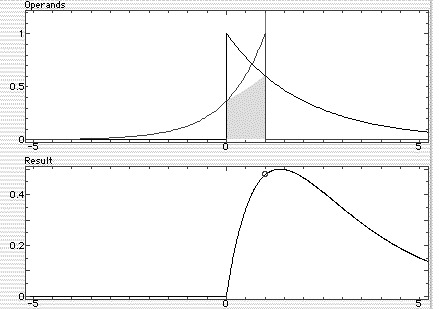
\includegraphics[width=\textwidth]{imgs/convolution.jpg}
\end{frame}

\begin{frame}[label=math-laplacian]{Laplacian}
 The Laplacian operator, or $\nabla^2$, is defined as the $n$-dimensional vector:
 \begin{equation}
  \langle 
   \frac{\partial}{\partial x_1},
   \frac{\partial}{\partial x_2}, \ldots
   \frac{\partial}{\partial x_n}
  \rangle.
 \end{equation}
 The Laplacian of $f$, or $\nabla^2 f$, is thus defined as:
 \begin{equation}
  \sum_{i=1}^n \frac{\partial^2 f}{\partial x_i^2};
 \end{equation}
 that is, the sum of the second-order partial derivatives of $f$.
\end{frame}

\begin{frame}
 \begin{itemize} 
 \item Suppose $f(x,y) = x^2 + y^2$. Then the Laplacian is:
 \item $\frac{\partial^2}{\partial^2_x} 
       (x^2 + y^2) +
        \frac{\partial^2}{\partial^2_x} 
       (x^2 + y^2) = 2+ 2 = 4$.
 \vspace{16pt}  
 \item Suppose $f(x,y) = x^2y^2$. Then the Laplacian is:
 \item $\frac{\partial^2}{\partial^2_x} 
       (x^2y^2) +
        \frac{\partial^2}{\partial^2_x} 
       (x^2y^2) = 2x^2 + 2y^2$.
 \end{itemize} 
\end{frame}


\begin{frame}[label=math-weierstrass]{Weierstrass Transform, or Gaussian Blur}
 The 2-dimensional Gaussian function is defined as follows:
 \begin{equation}
  G(x) = \frac{1}{2 \pi \sigma^2} e^{-\frac{x^2+y^2}{2\sigma^2}},
 \end{equation}
 the graph of which takes the shape of a bell. When a Gaussian is used to convolute an image $I$, the new pixel at $I(x,y)$ becomes the weighted average of all pixels in its neighborhood, producing a smoothing or blurring effect.
\end{frame}

\begin{frame}
\begin{center}
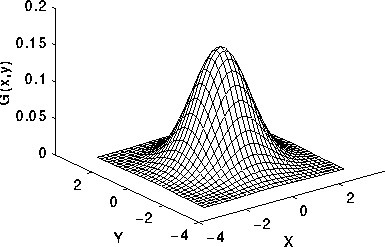
\includegraphics[width=\textwidth]{imgs/gauss.jpg}
\end{center}
\end{frame}

\begin{frame}[label=math-distance]{Euclidean and Mahalanobis Distances}
 \textbf{Euclidean distance}: for two given points $p_i$ and $q_i$, the Euclidean distance is:
  \begin{equation} \label{eq:euclidean}
   d(x,y) = \sum_{i=0}^{N} \sqrt{(p_i-q_i)^2}.
  \end{equation}
 \textbf{Mahalanobis distance}: for a given multivariate vector $x = (x_1, x_2 \ldots x_n)$ the Mahalanobis distance from a group of values with mean $\mu = (\mu_1, \mu_2 \ldots \mu_n)$ is defined as:
  \begin{equation} \label{eq:mahalanobis}
   D_M(x) = \sqrt{(x-\mu)^TS^{-1}(x-\mu)}.
  \end{equation}
\end{frame}

\begin{frame}
\begin{center}
 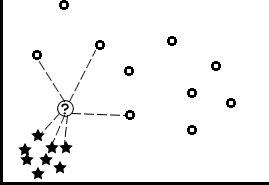
\includegraphics[width=.5\textwidth]{imgs/ex_euc_dist-fw.png}
 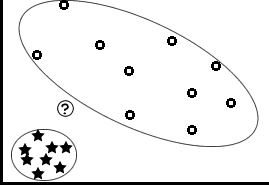
\includegraphics[width=.5\textwidth]{imgs/ex_mah_dist-fw.png}
\end{center}
\end{frame}

\begin{frame}[label=math-integral]{Integral Images}
 The integral image $I_\Sigma(x)$ at a location $\mathbf{x} = (x, y)^T$ is the sum of pixels in the input image $I$ within a rectangular region formed by the origin and $\mathbf{x}$:
 \begin{equation} \label{eq:integral}
  \sum_{i=0}^{i\leq x} \sum_{j=0}^{j\leq y} I(i,j).
 \end{equation}
\end{frame}

\begin{frame}

\begin{minipage}{.45\linewidth}
 \begin{center}
 \begin{tabular}{c|c|c}
  1 & 2 & 1 \\ \hline
  2 & 3 & 2 \\ \hline
  1 & 2 & 1 \\ \hline
 \end{tabular}
 \end{center}
\end{minipage}

\begin{minipage}{.45\linewidth}
 \begin{center}
 \begin{tabular}{c|c|c}
  1 & 2 & 1 \\ \hline
  2 & 3 & 2 \\ \hline
  1 & 2 & 1 \\ \hline
 \end{tabular}
 \end{center}
\end{minipage}

\end{frame}

\begin{frame}[label=math-frobenius]{Frobenius Norm}
The Frobenius norm $|A|_F$ of a matrix $A$ is simply defined as:
\begin{equation}
 \sqrt{\sum_{i=0}^n \sum_{j=0}^m A_{ij}^2}
\end{equation}
\end{frame}

\begin{frame}[label=math-clairaut]{Clairaut's Theorem}
 As a consequence of Clairaut's theorem:
 \begin{equation}
  \frac{\partial^2 f}{\partial x \partial y} = 
  \frac{\partial^2 f}{\partial y \partial x}.
 \end{equation}
 The analogous Young's theorem indicates that:
 \begin{equation}
 \end{equation}
\end{frame}

\begin{frame}[label=math-hessian]{Hessian Matrix}
Given a point $\mathbf{x} = (x,y)$ in an image $I$, the Hessian matrix 
\begin{equation}
\mathcal{H}(\mathbf{x}, \sigma) =
 \begin{bmatrix}
  L_{xx}(x,\sigma) &
  L_{xy}(x,\sigma) \\
  L_{xy}(x,\sigma) &
  L_{yy}(x,\sigma) 
 \end{bmatrix}
\end{equation}
where $L_{xx}(x,y)$ is the convolution of the Gaussian second-order derivative 
$\frac{\partial^2}{\partial x^x}g(\sigma)$ with the image $I$ in point $\mathbf{x}$; similarly for 
  $L_{xy}(x,\sigma)$ and
  $L_{yy}(x,\sigma)$.
\end{frame}

\end{document}
